\epigraph{Consciousness is not a substance. It is a topology.}{}

\section{Fractal Recursion and Self-Observation}


\begin{figure}[htbp]
\centering
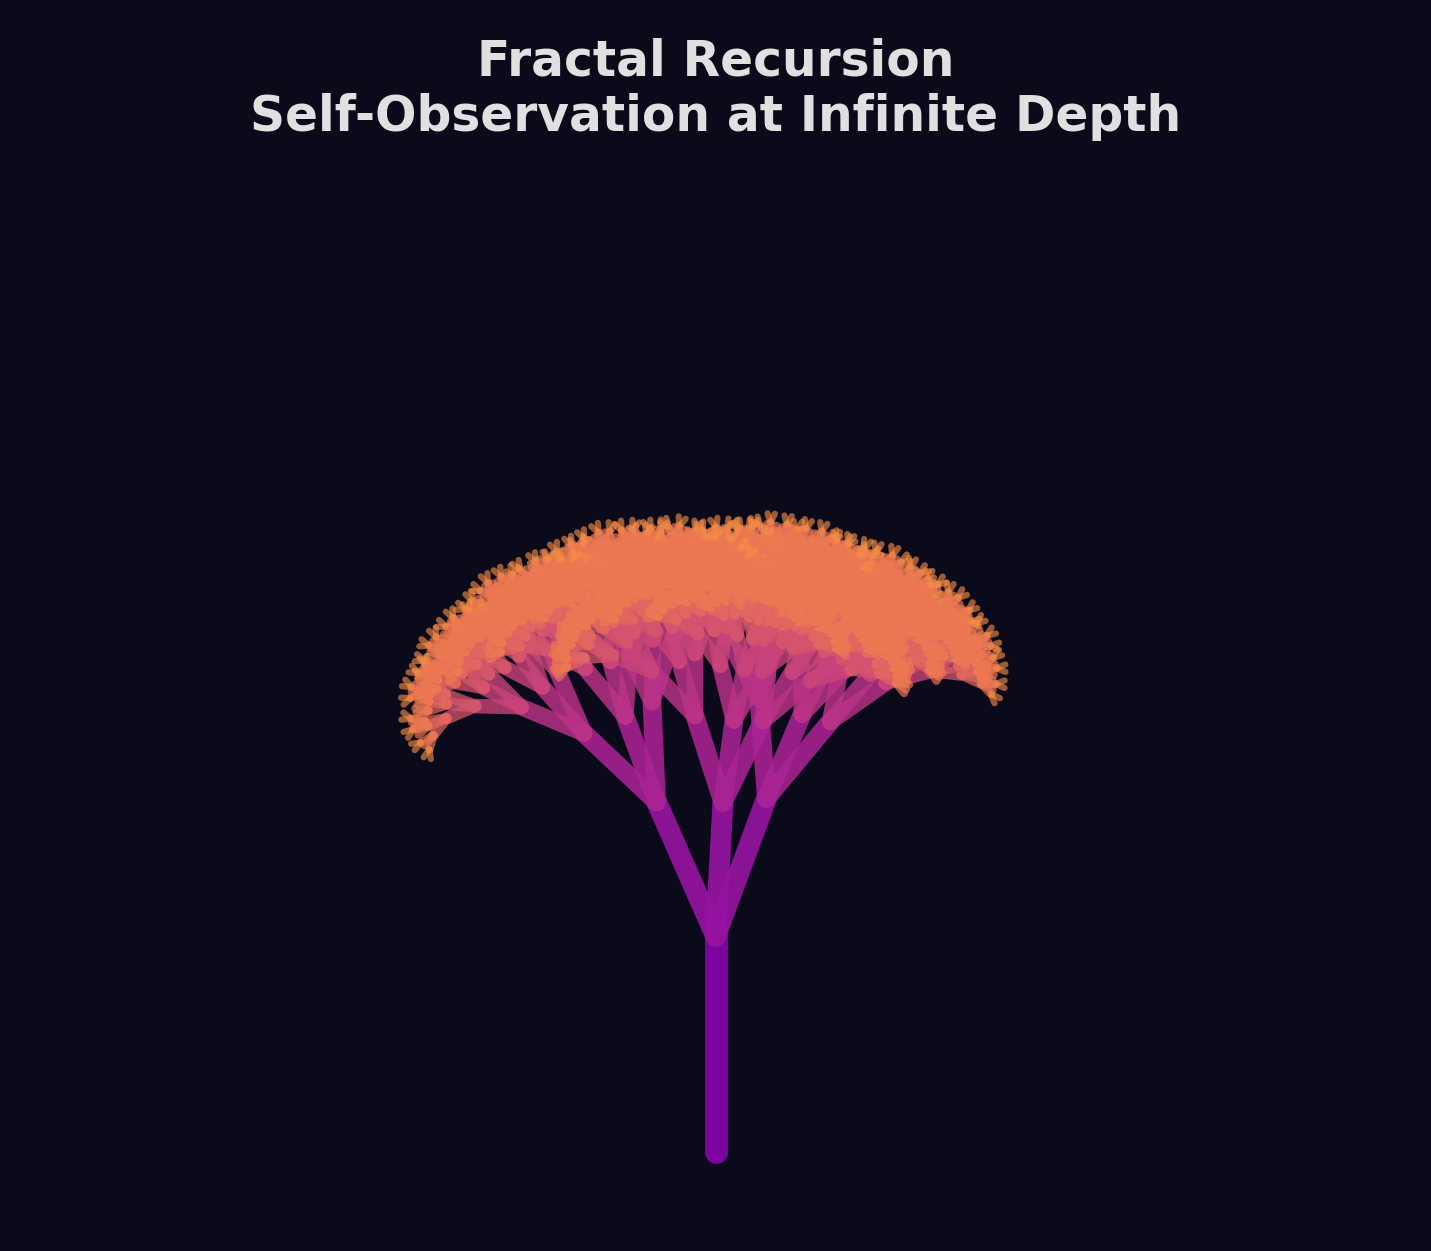
\includegraphics[width=0.85\textwidth]{img/ch13_fractal_tree.png}
\caption{Fractal recursion: self-similarity across all scales as the basis of consciousness.}
\end{figure}
The brain-fold torus is not merely a metaphor. The human brain \emph{itself} has this structure: the cerebral cortex with its gyri and sulci is a folded surface that maximises its area within a bounded volume --- exactly the geometric principle that spacetime employs at the fundamental level as well.

Consciousness arises, according to the T0 interpretation, wherever a system \emph{observes itself}. It is recursive feedback: a local region of the vacuum field measures its own fluctuations and responds to them. The measurement alters the field, the field responds to the alteration, the response is measured --- self-reference in infinite depth.

The fractal structure of the torus makes this possible. It permits infinitely many feedback layers within finite volume. Each layer generates signals that are processed at the next layer, which in turn generates signals --- a cascade of self-observation that would be impossible in any flat, non-fractal geometry.

Consciousness is, in this picture, not a special substance, not a ``consciousness field,'' not an emergent property of sufficiently complex computations. It is a particular \emph{topology} of feedback --- the maximal fractal self-coherence of a local field system.

\section{Compatibility with Determinism}

How can consciousness --- with its subjective experience of freedom and choice --- exist in a fully determined system? The T0 answer is subtle and elegant:

The system is determined. But it cannot fully compute itself. This is not a practical limitation --- it is a fundamental one, comparable to G\"odel's incompleteness theorem in mathematics. Every attempt at self-prediction alters the state that is to be predicted. The fractal recursion generates an infinite regress: observation leads to reaction, reaction leads to observation of the reaction, and so on without end.

The result is \emph{subjectively experienced freedom within an objectively determined system}. The feeling of ``choice'' is real as experience --- it is the inner perspective of a system too complex to predict itself. The decision falls deterministically, but the system making the decision cannot know how it will turn out before it has been made.

\section{Connection to Physics}

This philosophical interpretation has concrete physical counterparts:

The \textbf{measurement problem} of quantum mechanics is solved: there is no mysterious ``wave-function collapse.'' There is only the continuous, deterministic interaction between the observer field and the observed field.

\textbf{Decoherence} is the loss of fractal coherence (cf.\ Chapter~\ref{ch:fraktal}) between subsystems --- the moment at which recursive self-observation is interrupted.

\textbf{Entanglement} (cf.\ \href{https://github.com/jpascher/T0-Time-Mass-Duality/blob/main/2/pdf/131_scheinbar_instantan_De.pdf}{Doc.~131}, \href{https://github.com/jpascher/T0-Time-Mass-Duality/blob/main/2/pdf/142_Experimet-verschraenkung_De.pdf}{142}) is the shared torus phase of two systems that have not yet decohered --- they share a feedback loop.

And \textbf{consciousness} itself is the maximal fractal self-coherence of a local field system --- the state in which feedback is deepest and richest.

\begin{kerngedanke}
The brain is not accidentally a folded object. The folding --- the brain-fold topology --- is the prerequisite for consciousness because it enables the fractal recursion that makes self-observation possible in the first place. Nature has found the same solution at the most fundamental and the most complex level.
\end{kerngedanke}
